\section{Zadanie 19}
\begin{figure}[h!]
	\centering
	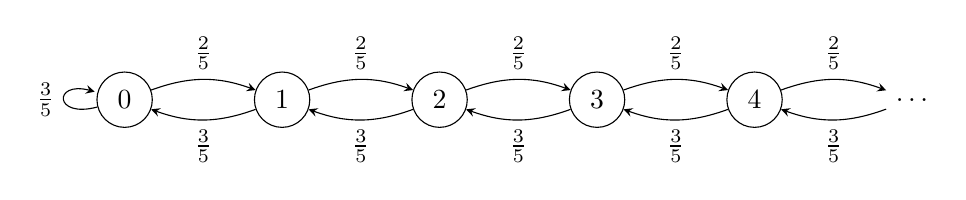
\begin{tikzpicture}[>=stealth, node distance=2cm, auto]
		\tikzstyle{state}=[circle, draw, minimum size=20pt]

		% nodes
		\node[state] (0) {0};
		\node[state, right of=0] (1) {1};
		\node[state, right of=1] (2) {2};
		\node[state, right of=2] (3) {3};
		\node[state, right of=3] (4) {4};

		% self-loop at 0
		\path[->] (0) edge[loop left] node {$\frac{3}{5}$} ();

		% transitions
		\path[->] (0) edge[bend left=20] node {$\frac{2}{5}$} (1);
		\path[->] (1) edge[bend left=20] node {$\frac{3}{5}$} (0);

		\path[->] (1) edge[bend left=20] node {$\frac{2}{5}$} (2);
		\path[->] (2) edge[bend left=20] node {$\frac{3}{5}$} (1);

		\path[->] (2) edge[bend left=20] node {$\frac{2}{5}$} (3);
		\path[->] (3) edge[bend left=20] node {$\frac{3}{5}$} (2);

		\path[->] (3) edge[bend left=20] node {$\frac{2}{5}$} (4);
		\path[->] (4) edge[bend left=20] node {$\frac{3}{5}$} (3);

		\node[,right of=4] (5) {$\dots$};

		\path[->] (4) edge[bend left=20] node {$\frac{2}{5}$} (5);
		\path[->] (5) edge[bend left=20] node {$\frac{3}{5}$} (4);

	\end{tikzpicture}
\end{figure}


Czy zadany wyżej spacer \(\Gamma\) jest nieprzywiedlnym i nieokresowym
łańcuchem Markowa? Czy istnieje jego rozkład stacjonarny?
Na podstawie poprzednich wniosków wywnioskuj,
jaką wartość przyjmuje \(\ev{\tau_x^{+}}\).


\subsection*{Rozwiązanie}

Łańcuch \(\Gamma\) jest nieprzywiedlny bo z każdego stanu możemy dojść do każdego. Jest też nieokresowy bo okres \(0\) jest równy \(1\) (da się dojść z \(0\) do \(0\)  w 1 kroku więc gcd równa się \(1\)), a jako iż jest nieprzywiedlny to okres wszystkich stanów jest identyczny.\\

Chcemy znaleść rozkład stacjonarny \(\pi\). Z definicji rozkładu stacjonarnego mamy, że:\\
\(\pi_0 = \pi_0 \cdot P(0,0) + \pi_1 \cdot P(1,0) = \pi_0 \cdot \frac{2}{5} + \pi_1 \cdot \frac{3}{5}  \implies \pi_1 = \frac{2}{3} \pi_0\)\\

Dla \(i>1\): \\
\(\pi_i = \pi_{i-1} \cdot P(i-1,i) + \pi_{i-1} \cdot P(i+1, i) = \pi_{i-1} \cdot \frac{2}{5}+ \pi_{i-1} \cdot \frac{3}{5}\)

Z tego równania, można się domyśleć, że jak coś ma je spełniać to coś w postaci \(\pi_i =\pi_0 \cdot r^i\). Jak podstawimy \(\pi_i = \pi_0 (\frac{2}{3} ) ^i\) co sugeruje nam to pierwsze równanie to okazuje się że drugie też jest spełnione. Pozostaje policzyć \(\sum_{i = 0}^{i=\infty} \pi_i = 3\pi_0\). Suma musi być jeden więc \(\pi_o = \frac{1}{3}\), a \(\pi_i = \frac{1}{3}(\frac{2}{3})^n\) działa jako rozkład stacjonarny.\\

Tej wartośćci oczekwianej nwm jak wyliczyć ale chat mówi że jest to \(\frac{1}{\pi_x}\) xd

